Některé vhodné případy použití byly definovány v průběhu textu. V této sekci se zaměřím na obecné příklady použití, respektive na modelování základních vhodných situacích, poté bych shrnul zajímavé případy použití, které světově významné firmy používající Cassandru prezentovali na Cassandra Summitu 2013 v Londýně, kterého jsem se zúčastnil. V poslední části této kapitoly bych se chtěl věnovat případům využití, které jsem sám použil ve své praxi a nebo navrhoval v analýzách projektů. 

\section{Obecné modelování}

\subsection{Jednoduché struktury s nesloženým primárním klíčem (Statické tabulky)}

Pokud struktura dat nevyžaduje žádné složité operace a dotazy a vystačíme si s modelem kde klíč je tvořen jedním sloupcem tedy například pouze nějaký hash, můžeme použít jednoduchou definici tabulky jako v \ref{CQL1}. Z této tabulky pak jednoduše dta čteme i zapisujeme tak, jak jsme zvyklí z klasického SQL.

\subsection{Struktury se složeným primárním klíčem (Dynamické tabulky)}

Dříve než popíšeme jakým způsobem je možné vytvářet dynamické tabulky je potřeba vysvětlit jak cassandra zachází s se skládáním primárních klíčů

\subsubsection*{Složené klíče}
V Cassandře můžeme skládat klíče na 2 části (ty mohou byt tvořeny jednim sloupcem, nebo opět složenými sloupci), První část klíče se nazýva partition key a určuje, z čeho se bude skládat interní primární klíč, tedy ten co se hashuje a následně distribuuje po clusteru. Druhá část klíče se nazývá clustering key, který automaticky na daných sloupcích vytváří index a řadí data dle těchto sloupců. Interně slouží tyto sloupce jako prefix v názvech ostatních sloupců a fragmentuje podle nich data uvnitr jedné řádky. 

\begin{lstlisting}[caption={Ukázka složených klíčů},label=CQL2]
CREATE TABLE Cats (
  block_id uuid,
  breed text,
  color text,
  short_hair boolean,
  PRIMARY KEY ((block_id, breed), color, short_hair)
);
\end{lstlisting}

Příklad \ref{CQL2} říká že Partition Key je složený ze sloupců \emph{block\_id} a  \emph{breed} a clustering sloupce jsou \emph{color} a \emph{short\_hair}. Cassandra uloží data, která mají stejný \emph{block\_id}, ale jiný \emph{breed} na jiný uzel než data, která mají hodnoty těchto sloupců stejné.  


\subsubsection*{Časosběrné události 1}
Ideálním příkladem na ukázku toho, jak se používají složené klíče respektive implementace dynamických tabulek, tedy využití vlastnosti Cassandry, že v Column family nemusí mít pevný formát sloupců, jsou časosběrné události. Ukládáme různé hodnoty v čase na různých místech nebo pro různé uživatele. Ukázkový příklad sbírá data na meteorologických stanicích, a ukládá aktuální teplotu pro daný čas.

\begin{lstlisting}[caption={Dynamická tabulka 1},label=CQL3]
CREATE TABLE temperature (
   weatherstation_id text,
   event_time timestamp,
   temperature text,
   PRIMARY KEY (weatherstation_id,event_time)
);
\end{lstlisting}

Jako primární klíč jsme zvolili id stanice, které bude tvořit také interní klíč pro Cassandru a čas události, což bude název sloupce který bude mít hodnotu aktuální teplotu. Sloupce se interně budou automaticky řadit podle času. Interně tedy bude následujícíc tabulka vypadat následovně. 

\begin{figure}[h]
\centering
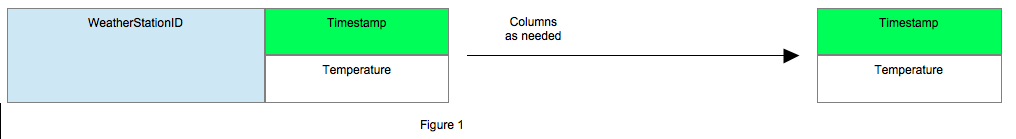
\includegraphics[scale=0.4]{images/timeseries1}
\caption{Interní reprezentace dat tabulky \ref{CQL3}}
\label{fig:timeseries1}
\end{figure}

Jak je z obrázku \ref{timeseries1} patrné, tímto formátem využíváme zmíněnou výhodu o odlišné struktuře řádek v Colum Family. Každá meteostanice má vlastní řádek a sloupce tvoří časové razítko kdy byla naměřena daná hodnota. Časové razítka mohou být samozřejmě pro každou stanici jiná a tudíž bude mít i každá řádka odlišné sloupce. Takto můžeme data jednoduše vkládat a dotazovat se nadnimi. V případě časosběrných událostí máme ovšem jednu nevýhodu jsme limitování maximálním počtem sloupců, který je sice asi 2 miliardy, ale pokud uvážíme, že bysme data měrili každou milisekundu, dojdou nám sloupce dřív než za měsíc.  

\subsubsection*{Časosběrné události 2}
U předchozího řešení jsme narazili na problém, kdy nám mohou dojít sloupce pro danou řádku. Řešení tohoto problému je celkem jednoduché, použijeme při navrhování modelu vzor, rozdelení řádky kdy první část primárního klíče (Partition key) složíme ze dvou sloupců stejně jako v ukázce \ref{CQL2}.


\begin{lstlisting}[caption={Dynamická tabulka 2},label=CQL4]
CREATE TABLE temperature_by_day (
   weatherstation_id text,
   date text,
   event_time timestamp,
   temperature text,
   PRIMARY KEY ((weatherstation_id,date),event_time)
);
\end{lstlisting}

Tabulku jsme upravili tak, že jsme přidali sloupec \emph{datum}, který zároveň tvoří partition key. Data se budou ukládat pro každou stanici a každý den data do samostnatné řádky, čímž je limit 2 miliardy sloupců vyřešen, protože v našem případě počítáme, že jedna stanice nebude denně provádět více než 2 miliardy měření. Interně to bude vypadat tak, že spojíme id stanice a datum, z této hodnoty se vytvoří interní row key a ten rozhodne na který uzel se data uloží. Schéme se změní následovně. 

\begin{figure}[h]
\centering
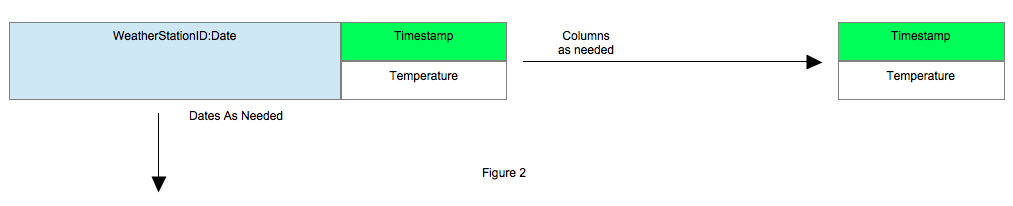
\includegraphics[scale=0.4]{images/timeseries2}
\caption{Interní reprezentace dat tabulky \ref{CQL4}}
\label{fig:timeseries1}
\end{figure}

Jak je vidět z předchozího příkladu, návrh a struktura dat se musí opravdu dobře rozmyslet předem, případné chyby v návrhu, jako opomenutí limitů se poté řeší velice nepřijemně. Komplikovanější návrh nezabere implementačně moc času navíc a bude fungovat pořád.


\subsection{Mixování Statických a dynamických tabulek}
Cassandra nativně umoňuje i mixování předchozích vzorů. Například máme dynamický prvek \emph{tag}, který přiřazujeme k uživateli, jehož ostatní sloupce jako jméno,adresa atd. jsou obyčejná statická tabulka. Cassandra takovýto návrh řeší nativně pomocí kolekcí. Kolekce jsou datový typ v CQL, který umožňuje mít v jednom sloupcí více hodnot a pracovat s nimi. Cassandra nabízí následující typy kolekcí.

\begin{itemize}
\item Set - ADT množina
\item List - ADT seznam
\item Map - ADT tabulka
\end{itemize}

Každý typ kolekce obsahuje odpovídající operace a  chování, jaké se dá očekávat u těchto abstraktních datových typů. Kolekce se dají použít kdykoliv, kdy chceme do statického modelu přidávat konečný počet, malých hodnot u kterých dopředu neznáme jejich počet. Kolekce mají následující omezení. 

\begin{itemize}
\item Maximální množství objektů v kolekcí je 64 000.
\item Maximální velikost objektu v kolekci je 64Kb
\end{itemize}

\section{Jak Cassandru používají významné firmy a služby}

V této sekci bych rád popsal několik reálných případu užití Cassandry ve všeobecně známých firmách, či službách. Některé z těchto případů užití byly demonstrovány na Cassandra Summit 2014, které jsem se v rámci tvorby této práce zúčastnil a s některými techniky daných firem jsem o implementaci Cassandry v jejich řešení hovořil. 

\subsection{Spotify a hudební seznamy}
Spotify je jedním z největších hráčů na trhu online přehrávání hudby avšak Cassandru nevyužívá k ukládání informací o skladbách, či skladby samotné, jak by se mohlo na první pohled zdát. Ve Spotify používají Cassandru k ukládání seznamů skladeb. Takovýchto seznamů mají více než 1 miliardu a musejí řešit několik zádrhelů ohledne jejich kolaborativních úprav, protože seznamy mohou být editovatelné více uživateli nebo jedním uživatelem z více míst a nebo dokonce změny v offline režimu. 

Ve spotify si s touto výzvou poradili výborně. Každý playlist je vlastne verzovaný objekt s jednoduchými operacemi: \emph{MOV} posune pisnicku z nejakého místa na jiné. \emph{ADD} na vybrané místo vloží písničku. \emph{DEL} vymaže písničku ze seznamu. Každou takovouto operaci zaznamenávají se speciálním časovým razítkem a odkazem na předchůdce tohoto otce. Dále si v jiné CF ukládají odkaz na takzvaný \emph{HEAD} tedy poslední operaci. Díky souběžným změnám těchto hlaviček může být několik. Což vede k rozvětvení playlistu v určitém bodě. Pomocí algoritmů operačních transformací dokáží z libovolného místa seznam zreprodukovat a dokonce provézt sjednocení rozdělených větví. Cassandra je ty vhodná k použití kdykoliv, kdy potřebujeme uložri velké množství jakkoliv verzovaných objektů. 

\subsection{Netflix}
Netflix patří mezi nejvetší hráče v poli streamování video obsahu. Přestože se jedná o podobnou službu jako Spotify, tak využívají Cassandru na úplně jiná data. A to téměř všechna data. Netflix má po celém světě přes 30 milionů aktivních uživatelů a do Cassandry ukládají informace o uživatelích, metadata o veškerém video obsahu nebo dokonce statistiky. Zajímavostí je, že netflix nemá žádnou vlastní infrastrukturu a veškeré servery hostují přes službu Aazon AWS. Netflix je také jedním z velkých přispěvovatelů do zdrojových kódů Cassandry a převážně právě do sekce věnující se deployi a správě Cassandra clusteru na tuto službu od Amazonu. Tento případ užití by měl zviditelnit výhody ukládání plochých databázových struktur napříč několika datacentry po celém světě. 

\subsection{Ebay} 
Ebay je největší internetová aukční síň, která má desítky milionů uživatelů. Cassandru využívá na několik svých služeb. První z nich je unikátní doporučovací systém. Každý uživatel prochází desítky položek při hledání určitého zboží a na základě toho na které položky klikl nebo naopak neklikl Ebay ukládá veškeré tyto události formou grafu, který znazorňuje uživatele, nabízené zboží a vztahy mezi nimi. Díky tomuto systému může Ebay svým uživatelům nabízet stále přesnější výsledky. 

Ebay využívá také Cassandru na zpracovávání sociálních dat, jako jsou například zobrazení, přání a oblíbené položky. Tyto hodnoty pro jednotlivé produkty vždy napočítá pomocí MapReduce. 

Poslední případ na který v Ebayi Cassandru používají jsou v podstatě jakékoliv časosběrné události. Například:
\begin{itemize}
\item Mobilní notifikace jejich logování a sledování.
\item Sledování dat pro následné odhalování podvodů.
\item Analýza serverových logů a analytických dat.
\end{itemize}

Využití Cassandry v Ebayi ukazuje, další stránky využitelnosti například ohledně časosběrných požadavků. Ebay považuje za cassandru přínosnou hlavně z hlediska škálovatelnosti a množství zápisů, které souběžně dokáže. Ebay totiž za den provede do Cassandry 6 miliard zápisů.\cite{ebay} Ebay navíc používá ve všech svých clusterech DataStax Enterprise kvůli plné integraci s Hadoopem přes který provádí MapReduce. Schéma Ebay Cassandra cluster vypadá přibližně následovně.

\begin{figure}[h]
\centering
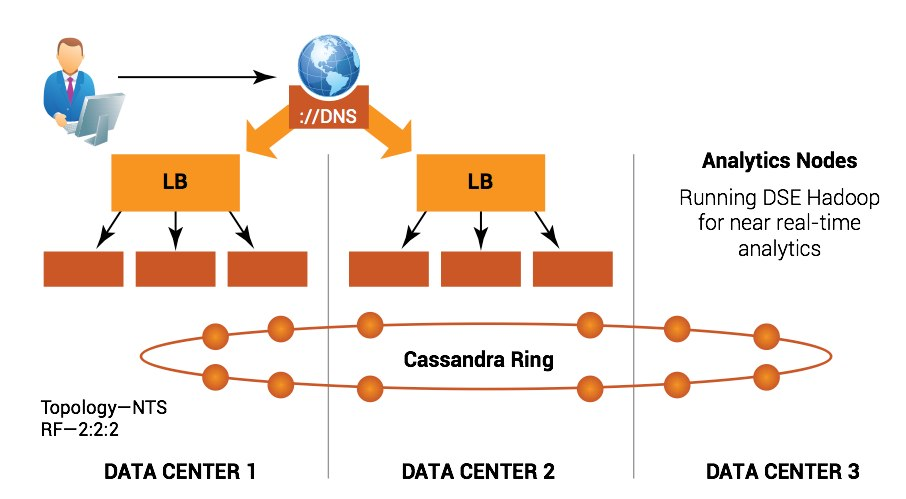
\includegraphics[scale=0.4]{images/ebay}
\caption{zdroj:  Cassandra at Ebay \cite{ebay}}
\label{fig:timeseries1}
\end{figure}

\subsection{Finn.no}
Finn.no je největší Norský webový server. Týdně přivítá 3.5 milionů návštěvníku v zemi, která má 5 milionů obyvatel. Jedná se o inzerční portál přes který lidé nabízejí, či poptávají realitní inzerci, pracovní pozice, věci na prodej, automibily, dovolené a služby. Na většinu z těchto oblastí mají v zemi monopol. Tento inzerční server Cassandru opět využívá na několik způsobů. Prvním je ohodnocení každé nabídky, která přijde a snaží se jí klasifikovat jako podvodnou. V případě podezření ji přepošle k manuální kontrole. Dále Cassandru využívají na implementaci zpráv mezi uživateli, což je vlastně originální případ užití a důvod vzniku Cassandry kdysi v kancelářích Facebooku. Cassandru zde využívají i na uchovávání uživatelovi historie hledání, kdy se uchovávájí jednotlivé informace o každém hledání a uživatel si může v profilu prohlédnout co hledal. V tomto případě se návrháři rozhodli, že jim stačí uchovávat data pouze za posledních 6 měsíců a proto využívají expirující sloupce, které po 6 měsících automaticky zmizí. Posledním případem využití je podobné sčítání zobrazení nebo přidání inzerátu do sledovaných jako na Ebay. Jednou za hodinu se spustí Hadoop Job, který pomocí MapReduce namapuje potřebné údaje, posčítá a následně uloží zpět do databáze a tak ve Finn.no počítají zobrazení inzerátu nebo sledování inzerátu. 

Zajímavostí na implementaci Finn.no je, že většina firem používá více menších strojů. Ve Finn.no mají pouze 6 uzlů s velice výkonným hardwarem a to kvůli lokalitě dat, která pro ně má mnohem větší cenu než drobné blokující IO operace. 

\section{Ostatní navržené případy užití}

V této sekci bych se na závěr kapitoly chtěl zaměřit na případy užití se kterými jsem přišel do styku v reálném prostředí nebo je teoreticky navrhoval pro nerealizované, či věděcké projekty. 

\section{Analýza Access logů}
První z těchto zajímavých případů užití se týká analýzy access logů. Dostal jsem za úkol navrhnout řešení, které by umožnilo velké nadnárodní společnosti s pobočkami po celém světě a více než 20 000 zaměstnanci monitorovat jaké weby její zaměstnanci navštěvují v pracovní době. Na základě těchto dat poté tvořit grafy a reporty pro konkrétní uživatele nebo oddělení. Součástí analýzy řešení byl i prototyp vybraného řešení. Seznam poždavků byl následující. 

\begin{itemize}
\item Možnost stahování či uploadu dat z acess logů do systému
\item Pro konkrétního uživatele či oddělení vyrobit report obsahující
\begin{itemize}
\item Zobrazovat data za vybrané časové období (1 týden až 6 měsíců zpět.) 
\item Zobrazovat navštívené stránky s absolutním číslem přístupů a procentuálním poměrem. 
\item Zohlednit příznak firewallu o statusu požadavku (OK, Podezřely, Nepřípustný)  
\end{itemize}
\item Data uchovávat pouze po dobu 6 měsíců. 
\item Data musí být přístupná ihned avšak klidně s denním zpožděním (logy se netahají z celého světa současně). 
\end{itemize}

Po sběru požadavků jsem ihned identifikoval, že toto je přímo ukázkový příklad pro využiží Cassandry. 

Tento případ užití jsem shledal natolik zajímavý a to jak zhlediska možností implementace, praktickým přínosem a významností, že jsem po domluvě s vedoucím práce tento případ využití využil i praktické části a závěrečné části této práce, kde ho dopordobna rozeberu.

\section{Obrázkové Servery}
Dalším zajímavým případem využití se kterým sem setkal je i příklad užití, kde se čtení provádí mnohonásobně častěji než zápis. Takovým způsobem je obrázkový server. V dnešní době mobilních zařižení je naprosto běžné, že potřebujete mít obrázek v několika velikostech. Vzhledem k rostoucímu počtu různorodých zařízení vznikají potřeby pro nová a nová rozlišení. Na toto můžeme využít Cassandřinu vlastnost nepevného schématu. Pro každý obrázek, uložíme originální velikost včetně metadat a při dotazu na konkrétní obrázek vytáhneme z databáze příslušný obrázek. Samozřejmě by bylo vhodné doplnit o nějakou vrstvu cachování. Tento use case je velice praktický a komplexní jelikož závisí na ostatním nedatabázovém softwaru a proto jsme po konzultaci s vedoucím práce rozhodli obrázek zařadit. Podobným způsobem uchovávál své obrázky například facebook, než napsal vlastní specifický systém na správu fotografií na hodně nízkoúrovňové úrovni. 

\section{Sběr a vyhodnocení transakčních událostí}
V maloobchodě je běžné zjišťovat oblíbenost produktů a hledání vazby mezi jednotlivými předměty a uživateli. Ukládáním všech transakcí a přiřazováním je ke konkrétním uživatelům (například v E-Shopu, nebo pomocí věrnostní karty).Správnou manipulací s daty, jsme schopni vymodelovat například následující grafy.

\begin{itemize}
\item Uživatelé co zakoupili produkt X také zakoupili tyto produkty.
\item Graf uživatelů, kde hrany reprezentují vazbu alespoň jednoho společně zakoupeného předmětu a ohodnocení hrany znamená počet takovýchto předmětů. 
\end{itemize} 
Předchozí grafy lze také upravovat změnou množiny předmětů a sledovat změny na základě určité skupiny předmětů. Takovéto grafy dokáží odhalit vazby mezi předměty, ale také vazby a podobnost mezi uživateli a předpovídat jejich další aktivitu. 
\newpage
\section{Hledání korelací}
Pokud máme dostatek dat, můžeme se mezi dvěma veličinami snažit o hledání kovariance, respektive korelačního koeficientu mezi těmito veličinami. Veličinou myslíme data hodnotu dat v čase. Například každý den ukládáme, kolik jsme prodali kusů kterého zboží, jaká je teplota, jaký je aktuální kurz měny atd. A můžeme pak jednoduše hledat spojitosti například mezi počasím a počtem prodaného zboží. Nebo vztah 2 různých prodávaných artiklů mezi sebou. Pro obchodníky jsou poté tato data velice důležitá a pomáhají jim lépe pochopit myšlení svých zákazníků a předpovídat jejich chování a také lépe plánovat provoz svého podnikání. Tento případ užití si ve zjednodušené podobě popíšeme i v následující kapitole. 

\section{Podpora v plně distribuované síti}
Ing. Josef Gattermayer vede výzkumný projekt, zabývající se plně distribuovaným systémem na rozesílání zpráv mezi uzly. Tento projekt se zatím řeší pouze v teoretické rovině a jeden z problémů který je potřeba vyřešit je notifikování uzlů, které byli offline, že na ně někde čeká zpráva. 

V tomto ohledu jsem se nechal inspirovat vlastností Cassandry, kterou používá při zapisování a to konrétně, Hinted Handoff, který byl popsán v předchozích kapitolách. Tento návrh předpokládá, že cluster je z hlediska infrastruktury jednotlivých uzů a služeb na nich běžících, nehomogení. Návrh zpočívá v tom, že přestože by si všechny uzly byly rovné po stránce komunikační, některé uzly by byly zároveň uzly perzistentními, které by ukládaly informace například do Cassandry. Tyto perzistentní uzly by zpravidla měly být nějaké serverové stanice, u ostatních komunikačních uzlů se nemusíme omezovat pouze na servery a můžeme počítat i se zařízeními jako jsou mobilní telefony, či přenosné počítače. Komunikační proces by v případě neúspěšného doručení zprávy byl následující. 

\begin{enumerate}
\item Uzel A vyšle zprávu pro uzel B
\item Uzel C zjistí nedoručitelnost, protože uzel B je nedostupný.
\item Uzel C kontaktuje jeden z perzistentních uzlů a zprávu do něj uloží s určitou dobou platnosti. 
\end{enumerate}

Při příchodu uzlu B zpět online. Provedou se následující operace.

\begin{enumerate}
\item Uzel B kontaktuje kterýkoliv perzistentní uzel s dotazem, zda-li pro něj má nějaké nedoručené zprávy.
\item Perzistentní uzel pošle pro něj uchovanou zprávu uzlu B.
\item Perzistentní uzel zašle zprávu o doručení uzlu A.
\end{enumerate}


V případě, že chceme dodržovat striktně distribuovanost informací, nebudeme na perzistentní server ukládat zprávy jako takové, ale budeme ukládat pouze takzvané hinty a operace budou probíhat následovně. 

\begin{enumerate}
\item Uzel A vysle zpravu pro uzel B
\item Uzel C zjistí nedoručitelnost, protože uzel B je offline.
\item Uzel C uzel zkontaktuje zpět uzel A, že zprávu nelze odelsat.
\item Uzel A uzel si zprávu uloží a zkontaktuje perzistentní server aby uložil hint pro uzel B.

\end{enumerate}

Při příchodu uzlu B zpět online. Provedou se následující operace.

\begin{enumerate}
\item Uzel B kontaktuje kterýkoliv perzistentní uzel s dotazem, zda-li pro něj má nějaké nedoručené zprávy.
\item Perzistentní uzel pošle uzlu B hint o tom, že uzel A pro něj má zprávu. 
\item Uzel C zasle uzlu A požadavek na znovuposlání zprávy.
\end{enumerate}


V obou předchozích scénářích předpokládáme, že uzel B se stane nedostupným, až po odeslání zprávy. Před odesláním zprávy si tuto informaci může zjistit uzel A sám a provede operace jako kdyby byl uzel C, aniž by zprávu někam posílal. Ve druhé variantě, je potřeba ošetřit problém cyklických hintů pokud uzly budou navzájem střídavě nedostupné a pro jednu zprávu by mohlo být uloženo nekonečně mnoho hintů. Pro daný pár uzlů nám vždy stačí mít uložen právě jeden hint pro daný směr požadavku. Tento případ užití je pouze teoreticky a měl by demonstrovat možnost využití distribuovaného systému jako je Cassandra v jiných distribuovaných systémech jako úložiště nebo monitorovací prvek tohoto systému. 


\chapter{Popis implementace vybraných případu užití}
V předchozí kapitole jsem popsal několik různých druhů užití Cassandry v reálných podmínkách. Vzhledem k zadání této práce, jsem po konzultaci s vedoucím práce, vybral jednoduchých a rozdílných případů, které budou sloužit jako podklady pro přípravu cvičení a laboratoří nově připravovaného předměnu na ČVUT.

\section{Testovací prostředí}
Součástí zadání bylo vypracovat tyto případy užití na školní infrastruktuře. Vzhledem ke komplikované instalaci a správě veškerého potřebného softwaru bylo z hlediska efektivity práce a oprávnění od této myšlenky upuštěno. Fakulta vlastní i experimentální výpočetní cluster a Tomáš Bartoň, kterému bych tímto chtěl poděkovat, mi nabídl řešení, které se zprvu zdálo dostačující, ale vzhledem ke komplikacím jsme i od tohoto řešení museli upustit. Finální implementace tedy proběhla na clusteru tvořeném z virtuálních strojů na jednom fyzickém počítači pomoci XENu. Pro Ing. Gattermayera, který předmět připravuje, jsem připravil XEN obraz, díky kterému lze vytvořit nový uzel a spustit na něm Cassandru. Toto řešení se ukázalo i pro garanta předmětu jako nejvhodnější a nejjednodušší. 

\section{Implementace Access Log analyzéru}
Jak bylo zmíněno v předchozí kapitole, dostal jsem za úkol vypracovat analýzu a prototyp řešení pro nadnárodní německou firmu zaměstnávající  více než 20 000 lidí po celém světě. Tito lidé se z firemní infrastruktury připojují do internetu a firma chce monitorovat návštěvnost stránek jednotlivých uživatelů a oddělení pro různá časová období, která však nejsou delší než 6 měsíců a na základě kriterií generovat online reporty. Tento zdánlivě jednoduchý problém v sobě ve skutečnosti skrývá několik netriviálních úkolů. Nejdříve je to především množství dat, které je potřeba zpracovat. Pokud bychom zpracovávali data sekvenčně tak bychom museli procházet približně 1860 GB systémových logů, což bychom rozhodně v žádné relační databázi nemohli provézt v rozumném čase. Data dostáváme inkrementálně kažýd den, vždy za předchozí den a to v několika dávkách z různých serverů po celém světě. 


\subsection{Návrh řešení pro ukládání všech logů}
Rozhodl jsem se že data budu ukládat do tabulky v Cassandře všechny data buud zapisovat s atributem TTL tak, aby sám za půl roku vypršel a data se automaticky smazala. Strukturu tabulky jsem navrhl následovně. 

\begin{lstlisting}[caption={Návrh tabulky pro ukládání všech logů},label=LogTable]
CREATE TABLE accesslog_ks.logs ( 
user text,
date timestamp,
webpage text,
severity text,
PRIMARY KEY (user,date) 
);
\end{lstlisting}

Sloupec \emph{severity} znázorňuje \uv{nebezpečnost} dotazu, tak jak to vyhodnotil proxy server. Tento údaj byl součástí analýzy a celý příklad značně komplikuje, jak bude vysvětleno níže. Jako primární klíč jsem zvolil návrhový vzor pro časosběrné údaje tedy, uživatele a časové razítko. Pro zjednodušení tohoto příkladu předpokládáme, že uživatel v jednu vteřinu nepřistoupí na více webových stránek. V reálném světě by bylo dobré do klíče přidat i webovou stránku, či zpřesnit časové razítko i na milisekundy. 

\subsection{Naivní řešení}
Prvním řešením jak získat data pro reporty je dotazování se přímo nad tabulkou logů. Nápad by se mohl zdát naprosto špatný, ale opak je pravdou. Jak dokládá následující tabulka, pokud by nám šlo o jedno konkrétní datum, je přístup do databáze velice rychlý i přes obrovské množství záznamů a prokazuje se, jak mocná Cassandra je. Čas nutný na přístup ke všem datům je na toto množství záznamů také výborný, avšak pro ještě větší záznamy bychom stále nedosahovali časů vhodných k online reportu. Navíc v této struktuře nemůžeme jednoduše třídit data a veškeré řazení a vyhodnocování bychom museli následně provádět v kódu, což by bylo velice zdlouhavé a neefektivní. nemluvě o situaci, kdy bychom dotazovali na různá oddělení a museli bychom provádět dotazů několik. Data v tabulce neodpovídají reálnému provozu, všechny uzly se nachází na jednom ne příliš výkoném počítači s jedním diskem, takže IO operace jsou velice limitované a následná komunikace s testovacím prostředím probíhá přes lokální síť. Reálné hodnoty by byly mnohonásobně nižší, cílem je poukázat na rozdíl hodnot v různých situacích.   	

\begin{table}[h]
%\begin{tabularx}{\textwidth}{ |l|l|l|l||| }

    \begin{tabular}{|l|l|l|l|l|}
    \hline
    \begin{tabular}{@{}c@{}}Počet \\záznamů \end{tabular} &  \begin{tabular}{@{}c@{}}Přibližný počet \\záznamů na uživatele \end{tabular} &  Vše [ms] & 1/3 [ms] & 1 den [ms] \\ \hline
    1000          & 200                                  & 160                  & 40                 & 20               \\ \hline
    11000         & 2000                                 & 600                  & 300                & 60               \\ \hline
    111000        & 20000                                & 3887                 & 1243               & 70               \\ \hline
    \end{tabular}
    \caption {Měření dotazování nad tabulkou logů}
\end{table}

\subsection{MapReduce 1}
Samozřejmě existuje lepší řešení, kterým je MapReduce data zredukujeme a uložíme do pomocné tabulky. Nejdříve projdeme schéma výsledné tabulky a následně si ukážeme mapovací a redukovací funkci.

\begin{lstlisting}[caption={Tabulka pro ukládání reportů},label=ReportTable]
CREATE TABLE accesslog_ks.reports ( 
user text,
webpage text,
date timestamp,
severity text,
count int,
PRIMARY KEY ((user,severity),date,webpage) 
);
\end{lstlisting}

Formát tabulky je zde téměř stejný jako v tabulce s logy, až na pár výjimek, sloupec \emph{date} nyni neoznačuje přesné časové razítko nýbrž pouze označení data bez času. Navíc zde přibyl sloupec count, který obsahuje informaci o celkovém počtu navštívení dané webové stránky pro tento den. Velice důležité je zde složení primárního klíče, které určuje jak se data budou ukládat a řadit uvnitř databáze. Důvody k výše uvedené skladbě klíče jsou následující. 

Kvůli jednoznačnému určení potřebujeme, aby klíč obsahoval všechny výše zmíněné atributy. Abychom se mohli dotazovat na konkrétní uživatele musí být uživatel partition key, respektive jeho první částí, abychom se mohli dotazovat na všechny nebo pouze na vybrané úrovně závažnosti, musí být jako druhá část partition klíče. Tato volba je prirozená, jelikož hodnota \emph{severity} nabývá konečného počtu předem známých hodnot a proto nebudeme tolik fragmentovat.Kdybychom \emph{severity} a \emph{user} prohodili, mohli bychom se sice ptát na více uživatelů, ale pouze na jeden konkrétní  stupeň závažnosti, což je v našem zadaní nelogické a neoptimální.

Po partition klíči následují další části primárního klíče a to datum, protože podle něj se budou výsledky uvnitř partition řadit, což je přesně to co chceme a navíc kdybychom \emph{date} a \emph{webpage} prohodili museli bychom se dotazovat na konkrétní weboou stránku abychom se vůbec mohli ptát na datum, což je vzhledem k funkcím aplikace nesmyslné. Jak je vidět, pořadí sloupců tvořící primární klíč je velice důležite! Takto složený klíč je pro námi zadaný příklad jediné správné a optimální řešení.

\subsubsection{Mapovací funkce}
Mapovací funkce je v tomto případě velice jednoduchá, musíme vytvořit univerzální schéma klíče abychom mohli sečíst návštevy v daný den. Proto potřebujeme datum  \uv{normalizovat}. V případě data nám stačí oříznout datum pouze na rok, měsíc a den. čas požadavku nás nezajímá. Z informací \emph{normalizovane datum}, \emph{adresa}, \emph{uživatel} a \emph{úroveň závažnosti} vytvoříme klíč ke kterému přiřadíme hodnotu 1, protože se jedná o jednu návštevu dané webové stránky v jeden den konkrétním uživatelem. 

\subsubsection{Redukovací funkce}
Redukovací funke je opět jednoduchá. Pro každý klíč provedeme sumu hodnot, tedy počtu navštívení a výsledek zapíšeme do výše uvedené tabulky s výše popsaným primárním klíčem, který se rovná stejnému klíčí, který jsme vytvořili v mapperu. 

\subsection{MapReduce 2}
V předchozím případě jsme viděli, jak napsat MapReduce job pomocí vlastního algoritmu, tedy nadefinování mapovací a redukovací funkce, v tomto případě to bylo relativně jednoduché a moc práce nám to nedalo, přesto je potřeba napsat několik tříd a vše správně zkompilovat a poté spustit. V druhém způsobu popíši, jak používat dotazovací jazyk Hive, který dotazy sám přeloží do MapReduce kódu, který spustí a vrátí výsledek. Tabulku na ukládání výsledků MapReduce jobů ponecháme stejnou jako v prvním případě, výsledek je totiž stejný. V jazyce Hive nám k předchozímu výsledku stačí pouze takovýto dotaz.

\begin{lstlisting}[caption={Tabulka pro ukládání reportů},label=Hive1]
select 
to_date(cast(logs.date as bigint)) as trimdate,
logs.user,
logs.webpage,
logs.severity, 
count(*) as count
from logs 
group by logs.webpage, logs.severity, logs.user,
to_date(cast(logs.date as bigint));
\end{lstlisting}

Tento dotaz vypadá složitě, ale je to jednoduchý SQL dotaz, který je programátorům využívajícím SQL velice blízký, jediná komplikovanější věc je funkce, která nám ořeže datum. Výsledkem tohoto dotazu jsou spočítané návštevy stránek, pro každý den pro všechny uživatele. Tento dotaz spustíme klasicky přes Hive JDBC konektor a její výsledky přes Cassandra JDBC konektor zapíšeme. A výsledek je stejný jako v předchozím případě s minimem psaní kódu, za cenu trochu delší doby běhu, než se vygeneruje MapReduce job. 

Hive experimentalne podporuje i vkládání do Cassandry přes externí tabulku. Kterou když vytvoříme, tak před dotaz \ref{hive1} vložíme příkaz \emph{INSERT INTO table}, kde table je název naší externí tabulky. Kod pro vytvoření a namapování tabulky vypadá následovně. 
\begin{lstlisting}[caption={Vytvoření externí tabulky napojené na tabulku v CQL},label=Hive2]
CREATE EXTERNAL TABLE hivereports (user string, webpage string,date timestamp, severity string, count int)
        STORED BY 'org.apache.hadoop.hive.cassandra.cql3.CqlStorageHandler'
        TBLPROPERTIES ( "cassandra.ks.name" = "accesslog_ks",
        "cassandra.cf.name" = "reports",
        "cassandra.ks.repfactor" = "2",
        "cassandra.ks.strategy" =
        "org.apache.cassandra.locator.SimpleStrategy");
		
ALTER TABLE hivereports SET TBLPROPERTIES ('cql3.output.query' = 'update accesslog_ks.reports set count = ? where user = ?  and webpage = ? and severity =?');
		
ALTER TABLE hivereports SET SERDEPROPERTIES ('cql3.update.columns' = 'user,webpage,date,severity,count');
\end{lstlisting}
Tento postup je ovšem opravdu experimentální a zatím nefunguje pro všechny případy a proto se jeho užití zatím obecně nedoporučuje. V případě napojení přes externí tabulku by nám tedy stačil jediny krátký dotaz a data by se nám uložila stejne jako v prvním případě. Nevýhodou ovšem zůstává, že takto nemůžeme použít TTL funkci při zápisu do Cassandry.

\subsection{Optimalizace}
Jednou možnou optimalizací, je omezení zadání, na před-definované celky času. Například 1den zpět, minulý týden nebo minulý měsíc, tedy že výběr data nebude libovolný, tím bychom snižili množství zápisů tabulky reportů a výběr těchto dat by byl rychlejší. 

Druhou a poněkud zásadnější optimalizací, je že v předchozích příkladech řadíme vždy z celé množiny dat, tomu můžeme předejít tím, že budeme MapReduce provádět pouze nad dnešeními daty, vzhledem k pravidelnému inkrementálnímu přírůstku dat, je tato optimalizace vhodná a nebudeme zbytečně pracovat s daty, která už mám jednou vypočítaná. 

\subsection{Skupiny Oddělení}
Součástí zadání je, že uživatel může chtít zobrazit souhrný report pro celé oddělení. V současné variantě bychom museli pro každého uživatele z oddělení udělat samostatný dotaz a výsledky spočítat, toto řešení je samozřejmě neefektivní. Pomůžeme si jednoduchým trikem, tabulku s logy rozšíříme o sloupec s informací o oddělení. A vytvoříme druhý MapReduce nebo Hive dotaz, který nebude brát v potaz sloupec s uživatelem, ale ten o oddeleni a v tabulce s logy budeme mít záznamy i o konkrétních odděleních. Nastane nám tím duplicita dat, která nám ovšem nevadí, jelikož je s ohledem na ostatní řešení nejmenší nevýhodou. 

\subsection{Statistiky}
V případě, že by uživatelé chtěli vidět souhrné statistiky jako počet navštívených stránek za včera (celkově), nebo nejoblibenejsi stránky obecně stačí pro každou z techto statistik vytvořit Hive dotaz, přesně pro takové účely je Hive ideální volbou. a výsledek uložit a následně zobrazovat v aplikaci. 

\subsection{Zhodnocení případu užití}
Tento případ považuji z hlediska praktického i názorného za velice užitečný a komplexní. Jedná se o rozsáhlý případ poukazující na několik technologií. Z hlediska využití tohoto případu v připravovaném předmětu, tento příklad se může použít na cvičeních věnujících se Cassandře, MapReduce, Hive. K porozumění je potřeba znalost mechanismů z přednášky. Vzhledem k rozsahu a komplexnosti jsme se s vedoucím práce dohodli, že tento případ bude hlavní a detailně rozepsaný a ostatní případy budou popsány a naimplementovány povrchově, aby došlo k poukázání základních principů použitých v daném případu. 


\section{Obrázkový server}
Tento případ užití poukazuje na moderní přístup k uchovávání obrázků a zároveň využití přístupu, kdy není pevně stanoveno schéma databáze. Přestože si vymodelujeme tabulku která pevnou strukturu má, interně se přeloží na bez schémový formát. Jedná se opět o reálný případ užití, který je používán a v současné době uchovává 7Gb dat. 

V dnešní době služby uchovávají velké množství obrázků a potřebují je zobrazit v různých velikostech. Posílání univerzálního obrázku na všechny dotazy je nevhodné, stejně tak jako zmenšování obrázku na základě každého požadavku. Ukládání obrázků přímo do filesystému přináší řadu nevýhod. Musí se řešit záloha a distribuovanost celého FS, kontrola konkrétních souborů a hlavně limity. Systém jako je Cassandra je víc než vhodný na tuto práci. Celý obrázkový systém se bude skládat z těchto částí

\begin{itemize}
\item Vrstva Cache na ukládání obrázků
\item Vrstva na úpravu obrázků 
\item Vrstva na ukládání obrázků a jejich čtení
\end{itemize}	


První dvě úrovně nás zajímají pouze teoreticky a záleží na konkrétních podmínkách jaké řešení bude v systému použito, cachování obrázků je velice užitečné, u často žádaných obrázků nikdy nedojde ke čtení z disku. Vrstva na úpravu obrázků oět záleží na konkrétní volbě v našem případě jakýkoliv software, či knihovna, která obrázek umí zmenšit. 

Co je pro nás mnohem důležitější je vrstva která obrázky ukládá a čte. Když dostaneme požadavek na obrázek, koukneme zda-li obrázek v této velikosti máme uložený v databázi. Pokud ano, vrátíme obrázek, pokud ne a obrázek ale máme v originální velikosti (tzn. obrázek evidujeme v databázi), obrázek zmenšíme na požadovanou velikost a vrátíme jej uživateli. Následně obrázek zpět uložíme do databáze s těmito rozměry a připravíme pro další použití. Pokud máme i cachovací vrstvu po vrácení obrázku je vhodné jej rovnou uložit i do cache. 

Schéma pro ukládání obrázků vypadá následovně. 

\begin{lstlisting}[caption={Tabulka pro ukládání obrázků v různých velikostech},label=img1]
CREATE TABLE images ( 
	id text,
	width int,
	height int,
	data blob,
	metadata text, 
	PRIMARY KEY (id,width,height) 
);
\end{lstlisting}

Primárním klíčem je identifikátor včetně velikosti obrázku. Data se tedy budou rozdělovat podle identifikatoru (první část primárního klíče). Slopec data bude obsahovat serializovany obrázek a sloupec metadata může obsahovat specifická metadata k tomuto obrázku. Pokud bychom chtěli pro všechny obrázky se stejným id udržovat jedny metadata, bylo by lepší pro metadata založit samostatnou tabulku. V případě, že každá velikost obrázku může mít jiná metadata, je tento návrh v pořádku. 

V aplikaci se poté jen dotážeme na obrázek v dané velikosti a vyhodnotíme výsledky způsobem popsaným výše. 

\section{Hledání korelací mezi daty}
V maloobchodě můžeme porovnávat například spojitost mezi prodejem dvou různých produktů nebo vliv počasí na prodeje. Jedná se o časo sběrnou událost, kdy za každý den ukládáme zisk za daný předmět (nebo počet prodaných kusů) tyto data můžeme získávat pomocí MapReduce z nějakého datasetu všech denních transakcí (například z ERP). Tabulku si vymodelujeme například takto. 

\begin{lstlisting}[caption={Tabulka zisků z prodeje předmětů v daný den},label=corr1]
CREATE TABLE sales ( 
	productId int,
	soldUnits int,
	date timestamp,
	revenue double, 
	PRIMARY KEY (productId,date) 
);
\end{lstlisting}

Nyní se můžeme dotázat na data pro 2 různé produkty za určité časové období a pomocí matematické knihovny, či tabulkového procesoru můžeme spočítat například korelační koeficient, který nám určuje provázanost mezi daty. Tento postup určitě není nic nového a jedná se zaběhnutou praxi, co je ovšem ale zajímavé a jaká možnost se nám díky BigData naskýtá, je že pomocí např MapReduce můžeme zkoušet hledat korelaci napříč všemi různými daty automaticky a když systém nalezne dobrý výsledek, oznámí vám to. Takto můžeme mezi svými daty hledat různé trendy. Je důležité si však uvědomit, že asociace dat neimplikuje kauzalitu. Na hledání trendů a korelací v uživatelských datech eixstují i  specializované firmy, které firmám s hledáním pomáhají, hledání těchto informací totiž není triviální.